%!TEX root = nucleare.tex
\part{Introduzione}
\chapter{Cenni storici}
\section{Planck - Quantizzazione dell'energia}
Sia\marginnote{12-11-1997} $S$ una sorgente radioattiva, cioè capace di emettere radiazioni. Queste radiazioni vengono classificate in base alla deviazione subita per effetto di un campo magnetico. Le radiazioni si chiamano, quindi:
\begin{itemize}
 \item[$\alpha$] nuclei di elio-4 $^4He^{2+}$;
 \item[$\beta$] elettroni $e^-$;
 \item[$\gamma$] fotoni. 
\end{itemize}

Secondo l'ipotesi di Planck, l'energia emessa da un corpo nero può assumere per ogni frequenza solo i valori \textit{discreti}
\begin{equation}\begin{split}
 W &= nh\nu\quad\text{con }n\in\mathbb{N}\quad\nu = \text{frequenza radiazione}\\
 h &= 6.6\times 10^{-34} \text{J s} \quad \text{costante di Planck.}
\end{split}\end{equation}

Un atomo si dice \textit{idrogenoide} quando ha un solo elettrone, quindi sono atomi ionizzati. Einstein avanzò un'ipotesi capace di spiegare completamente l'effetto fotoelettrico: questa era che l'onda elettromagnetica può trasferire agli elettroni solo quanti di energia (fotoni) secondo la formula
\begin{equation}
 \label{eq:energia_fotone}
 E = h\nu = cp
\end{equation}
in cui
\[
 \nu = \frac{c}{\lambda}\quad p = \frac{h}{\lambda}
\]
\section{Bohr - Quantizzazione del momento angolare}
Bohr ipotizzò la quantizzazione del momento angolare nell'atomo di idrogeno e negli atomi idrogenoidi secondo la formula
\begin{equation}
 \rvert\vec{L}\lvert = n\frac{h}{2\pi} = n\hslash
\end{equation}
Da questa ipotesi e applicando le leggi dell'elettrostatica al moto dell'elettrone, che si suppone circolare e descritto da leggi classiche, si deduce la \textit{quantizzazione delle orbite}. Cioè si ha
\begin{equation}
 r = n^2\frac{a}{Z}\,,\quad a=\frac{\hslash^2}{m_ee^2}\,,\quad e = 1.6\times 10^{-19}C
\end{equation}

L'energia associata a ciascuna di queste orbite è
\begin{equation}
 W = -\frac{Z^2e^2}{2a}\frac{1}{n^2}
\end{equation}
Bohr infine suppose che un atomo non irradiasse energia quando si trova in un determinato stato quantistico. Secondo la sua ipotesi, l'emissione di energia poteva avvenire solo con un passaggio dell'elettrone da uno stato all'altro. Supponendo quindi che l'elettrone passi da un'orbita $i$ a una $f$, la sua variazione di energia è
\begin{equation}
 W_i - W_f = - h\nu_{if}
\end{equation}
cioè la corrispondente variazione di energia viene convertita in un fotone con frequenza opportuna (se l'elettrone aumentasse la propria energia invece di emettere un fotone ne assorbirebbe uno). Dalla relazione di sopra si può ottenere un'espressione per le lunghezze d'onda che si possono avere. Si ha
\begin{equation*}
 \frac{Z^2e^2}{2a}\frac{1}{n^2_f}-\frac{Z^2e^2}{2a}\frac{1}{n^2_i} = h\frac{c}{\lambda_{if}}\qquad n_f < n_i
\end{equation*}
\begin{empheq}[box=\fbox]{equation}
 \frac{1}{\lambda_{if}} = \frac{Z^2e^2}{2ahc}\left(\frac{1}{n^2_f}-\frac{1}{n^2_i}\right)
\end{empheq}
Da questa espressione si ricava che
\begin{equation*}
 \lim\limits_{n_i\to\infty} \frac{Z^2e^2}{2ahc}\left(\frac{1}{n^2_f}-\frac{1}{n^2_i}\right) = \frac{Z^2e^2}{2ahc}\frac{1}{n^2_f}
\end{equation*}

Questa spiega il risultato sperimentale dell'addensamento delle righe spettrali negli spettri di emissione degli atomi di idrogeno o idrogenoidi. Questi risultati\footnote{Penso che una parola migliore sarebbe "formule", in quanto dovrebbe riferirsi a queste ultime.} sono tutti plasmati sui risultati sperimentali e non sono il risultato di una formulazione teorica. Quindi sono soggette a modifiche dovute ai miglioramenti degli esperimenti.

\section{De Broglie - L'ipotesi sulle particelle elementari}

De Broglie pensò di estendere il modello di onda-corpuscolo della luce anche alle particelle elementari. Estese quindi la validità delle relazioni \eqref{eq:energia_fotone} anche alle particelle. Per le onde elettromagnetiche si partiva dall'assodato modello ondulatorio per arrivare al modello corpuscolare. Per le particelle avvenne invece un processo inverso: dalla natura corpuscolare si arriva a quella ondulatoria, cioè ad una particella di cui siano noti $E$ e $p$ si associa un onda con $\nu$ e $\lambda$ ricavate dalle due relazioni di sopra. Per evidenziare la natura ondulatoria dell'elettrone è necessario farlo interagire con oggetti le cui dimensioni siano dell'ordine di grandezza della lunghezza d'onda dell'elettrone. Si usano per questo scopo i reticoli cristallini.

Osserviamo ora come dalle ipotesi di De Broglie si possa arrivare alla quantizzazione di Bohr. Infatti consideriamo un elettrone in un atomo: affinché la sua orbita sia stabile è necessario che questa sia costituita da un numero intero di lunghezze d'onda dell'elettrone. Cioè, se $r$ è il raggio dell'orbita deve valere $2\pi r= n\lambda$. Da questa, con semplici sostituzioni, si ritrova la legge $L = pr = nh/2\pi$.

Le prime particelle elementari studiate sono state l'elettrone, il neutrone, il fotone (anche se è una particella sui generis) e in un secondo tempo il positrone (protone)\footnote{È molto probabile che questo sia un errore. Non è infatti vero che positrone e protone sono la stessa cosa. Più probabile è che l'unica delle due sensata sia protone. [NdT]}. Oggi si contano circa un centinaio di particelle ed antiparticelle. Ad ognuna di esse si associa uno spin (momento angolare intrinseco): questo può assumere come valori soltanto \textit{multipli interi o seminteri di $\hslash$}.

Oggi si ritiene che i componenti ultimi della materia siano \textit{quarks e leptoni}.

\chapter{Apparati rilevatori}
Per\marginnote{12-11-1997} studiare proprietà e comportamenti di nuclei e
particelle è necessario rivelarli. Per tale motivo si usano apparati rivelatori
che segnano il passaggio delle particelle.

Un apparato deve essere \textit{sensibile agli effetti generati dalle
particelle} e inoltre deve ingigantire tali effetti per portarli dalla scala
microscopica alla scala macroscopica.

Le particelle cariche si rivelano tramite gli effetti prodotti per interazione
elettromagnetica con la materia circostante. Questa interazione si estrinseca
nella \textit{ionizzazione} della materia circostante, con una conseguente
perdita di energia da parte della particella carica in esame. Questa
progressiva perdita di energia causerà il rallentamento e infine l'arresto
della particella carica. Il cammino percorso da questa particella sarà
caratterizzato da un notevole numero di particelle ionizzate. I rivelatori
quindi mettono in risalto le particelle ionizzate.

\section{Tipi di rivelatori}

Esistono due tipi di rivelatori: \textit{visuali} e \textit{non visuali}. Nei
primi le cariche della materia ionizzata vengono usate per produrre effetti
visibili che permettono anche di eseguire delle fotografie della traiettoria
della particella. Nei secondi invece le cariche generate vengono usate per
ottenere \textit{impulsi elettrici}. Questi vengono poi opportunamente
analizzati mediante apparecchiature elettroniche. L'elemento comune dei due
tipi di rivelatori è la formazione di cariche di ionizzazione.

Al primo tipo di rivelatori appartengono le emulsioni fotografiche, la camera
di Wilson (a nebbia) e la camera a bolle. Al secondo tipo appartengono la
camera d'ionizzazione, il contatore proporzionale, il contatore Geiger-M\"uller
e il contatore a scintillazione.

Il metodo di rivelazione di tali apparati non può più essere efficace qualora
la particella da studiare \textit{sia neutra}. In questo secondo caso
\textit{le interazioni} con la materia circostante non sono di tipo
elettromagnetico e \textit{non sono sufficientemente intense e continue}.
Quindi gli unici metodi per rivelare particelle neutre sono indiretti e non si
potrà avere alcuna informazione sulla traiettoria della particella stessa. Si
potranno avere foto della traiettoria solo nel caso in cui
\textit{la particella neutra decada}, producendo per disintegrazione particelle
cariche. Per esempio in una camera a nebbia si potrebbero osservare le
traiettorie delle due particelle ottenute per
disintegrazione\footnote{O dalla sua rara interazione con la materia. [appunti
sugli appunti. Ah, l'ironia. NdT]}.

Gli apparati rivelatori sono usati insieme a degli acceleratori di particelle
che generano fasci di particelle. In genere tali fasci vengono fatti collidere
con la materia (sostanza bersaglio) o con altri fasci. I rivelatori osservano
quindi il risultato di queste collisioni. Esistono due principali motivi per
cui \textit{sono necessarie alte energie}:
\begin{enumerate}
 \item dalla meccanica quantistica sappiamo che per indagare su scale molto piccole bisogna lavorare con lunghezze d'onda molto piccole e per ottenere lunghezze d'onda molto piccole, dalla relazione di De Broglie $\lambda = h/p$, \textit{sono necessarie quantità di moto molto elevate};
 \item dalla teoria della relatività, più precisamente dal principio di equivalenza massa-energia, segue che \textit{particelle con grande massa devono avere molta energia}, quindi occorre \textit{molta energia per perturbarle significativamente}\footnote{Particelle pesanti tipo Bosone di Higgs [altro appunto sugli appunti. NdT]}.
\end{enumerate}
Analizziamo ora più in dettaglio i rivelatori a cui si era accennato.
\subsection{Rivelatori visuali}
\subsubsection{Lastre ad emulsione}
Questo è uno dei più importanti rivelatori visuali. Queste sono \textit{lastre i cui elementi sensibili sono granuli d'argento}.

Quando una particella carica attraversa una lastra ad emulsione si ha l'annerimento dell'emulsione (questo metodo è servito per i raggi cosmici)\footnote{Si rivelarono nel 1896-1898 i raggi $\alpha$ e i raggi $\beta$ con questo metodo.}.
\subsubsection{Camera di Wilson (o a nebbia)}

Anche questo è un rivelatore visuale. Questa consiste sostanzialmente di un recipiente pieno di gas e vapore acqueo che può essere espanso rapidamente tramite un pistone in maniera adiabatica. Questa espansione adiabatica provoca un raffreddamento ed in più il vapore risulterà soprasaturo. Se nel frattempo la camera è attraversata da una singola particella carica si formerà lungo il suo percorso una catena di atomi ionizzati che agiranno sul vapore come delle impurità ovvero dei veri e propri nuclei di condensazione\footnote{Come nelle nuvole con le goccioline attorno al pulviscolo. }. Attorno agli atomi ionizzati si formano quindi goccioline di acqua che danno una traccia visibile del percorso della particella.

Il meccanismo di espansione può essere azionato a intervalli regolari o in sincronia con l'uscita di fasci di particelle dell'acceleratore. Ovviamente la camera a nebbia (= di Wilson) funziona solo durante la fase di espansione.

\`E possibile comunque costruire camere a nebbia che funzionino in modo continuo, cioè senza un meccanismo di espansione. Consideriamo ad esempio un recipiente con del vapore acqueo e gas, con un gradiente di temperatura: in basso freddo e in alto caldo. Si genera così anche uno strato in cui il vapore è sempre soprasaturo e in grado di generare delle tracce.

\subsubsection{Camera a bolle}

Questo è un rivelatore visuale ed è un pò l'\textit{inverso}\footnote{\textit{Meccanismo speculare.} } della camera a nebbia. Esso è costituito da un recipiente pieno di un liquido a temperatura leggermente inferiore a quella di ebollizione. Se la pressione viene improvvisamente diminuita il punto di ebollizione si abbassa. In queste condizioni si ha la formazione di bollicine soprattutto attorno agli atomi ionizzati. Queste bollicine possono essere rese visibili tramite una \textit{intensa illuminazione}, quindi diventa possibile individuare la traiettoria della particella carica. Si consideri inoltre che si ha anche un processo di \textit{amplificazione} in quanto col passare del tempo le bollicine aumentano di volume.

\subsection{Rivelatori non visuali}
Analizziamo ora alcuni rivelatori non visuali.
\subsubsection{Camera di ionizzazione}

Questo è il più antico rivelatore. È costituito da un recipiente pieno di gas con due elettrodi a una data differenza di potenziale. Supponiamo che una sola particella carica attraversi la camera d'ionizzazione producendo un certo numero di ioni positivi e negativi. Il campo elettrico indirizzerà verso il catodo gli ioni positivi e verso l'anodo quelli negativi. Misurando la correte d'ionizzazione è possibile risalire all'energia iniziale della particella ionizzante. D'altra parte poiché gli elettroni prodotti nella ionizzazione saranno molto più veloci degli atomi ionizzati si può supporre che nell'intervallo di tempo che impiegano gli elettroni a raggiungere il catodo gli atomi ionizzati si siano appena mossi. Durante questo brevissimo intervallo di tempo il potenziale agli elettrodi subirà una variazione $\Delta V = \Delta Q / C$, dove $C$ è la capacità degli elettrodi e $\Delta Q$ è la carica depositata. L'impulso elettrico $\Delta V$ così ottenuto darebbe un segnale del passaggio della particella ionizzante. Di fatto però in una camera di ionizzazione pura e semplice questo impulso è molto piccolo e non consente di rivelare a una a una le particelle ionizzanti.

\subsubsection{Contatori proporzionali e di Geiger-M\"uller}

Questi rivelatori si basano sullo stesso principio su cui si basano le camere d'ionizzazione. In più però questi posseggono un dispositivo di moltiplicazione degli elettroni liberi. Questo amplifica il segnale elettrico e rende quindi possibile \textit{contare una alla volta} le particelle ionizzanti.

\subsubsection{Contatori a scintillazione}

Il principio di base su cui si fondano questi contatori è la \textit{emissione di quanti di luce} da parte di una molecola o di un reticolo cristallino stimolati dal passaggio di una particella ionizzante\footnote{Carica }. Si adoperano sostanze \textit{fluorescenti} in modo tale da evitare che la luce emessa sia immediatamente assorbita.

I primi contatori a scintillazione erano schermi ricoperti da solfuro di zinco ed erano adoperati come contatori visuali. Infatti la scintillazione generata sullo schermo si poteva osservare tramite un microscopio. Oggi invece tali contatori vengono utilizzati in un modo non visuale: il segnale sullo schermo viene amplificato tramite fotomoltiplicatori. Questi sono dispositivi che sfruttando l'effetto fotoelettrico trasformano poche decine di fotoni entranti in una valanga di fotoni uscenti.

Una caratteristica fondamentale di tali contatori è la loro \textit{prontezza}, che permette di \textit{individuare l'istante in cui passa la particella}\footnote{Elevato potere risolutivo temporale. }. In questo senso tali contatori possono considerarsi l'opposto delle emulsioni fotografiche che non danno informazioni sull'istante in cui è passata la particella carica ma danno un segnale permanente.

\chapter{Processi dinamici}

In fisica\marginnote{14-11-1997} nucleare e subnucleare esistono sostanzialmente
due tipi di processi dinamici: i processi di diffusione (o di
\textit{scattering}) e i processi di decadimento.

\section{Processi di diffusione}

Un tipico processo di diffusione si ha quando un fascio di particelle incidenti
con velocità $v$ attraversa uno strato sottile in cui sono presenti delle
particelle bersaglio in quiete. Al seguito dell'interazione il fascio viene
diffuso in diverse direzioni.

Le particelle bersaglio sono tutte identiche fra loro e così anche le particelle incidenti.
\begin{wrapfigure}{l}{4.872cm}
  \caption{Bombardamento di lamina bersaglio e diffusione successiva.}
  \label{fig:diffusione}
  \begin{tikzpicture}[line cap=round,line join=round,>=triangle
  45,x=1.0cm,y=1.0cm]
  \clip(-0.04,-1.89) rectangle (4.32,3.91);
  \draw [->,color=\MainColor] (0,1.5) -- (2,1.5);
  \draw [->,color=\MainColor] (0,2) -- (2,2);
  \draw [->,color=\MainColor] (0,1) -- (2,1);
  \draw [->,color=\MainColor] (0,0.5) -- (2,0.5);
  \draw [->,color=\MainColor] (0,0) -- (2,0);
  \draw (2.5,2.5)-- (2.5,-0.5);
  \draw [->,color=\SecondaryColor] (2.5,2.76) -- (2.5,3.9);
  \draw [->,color=\SecondaryColor] (3.1,2.1) -- (4.18,2.8);
  \draw [->,color=\SecondaryColor] (3.18,1) -- (4.32,1);
  \draw [->,color=\SecondaryColor] (3.1,-0.1) -- (4.18,-0.8);
  \draw [->,color=\SecondaryColor] (2.5,-0.76) -- (2.5,-1.9);
\end{tikzpicture}

\end{wrapfigure}
Quando la singola particella incidente e la singola particella bersaglio dopo l'urto non hanno subito alcuna variazione interna si parla di \textit{diffusione elastica}. Quando invece avvengono delle variazioni interne si parla di \textit{diffusione anelastica}\footnote{Processo di reazione. }.

Le grandezze importanti sono la \textit{frequenza di diffusione} (o anche di transizione) e la \textit{sezione d'urto}. Si chiama \textit{evento} la diffusione di una singola particella incidente per effetto di una singola particella bersaglio. Si suppone che \textit{sia le particelle incidenti che quelle bersaglio siano insiemi statistici} e che le particelle incidenti \textit{arrivino perpendicolarmente al piano}.

Si\marginnote{Frequenza di diffusione} dice \textit{frequenza di diffusione} il numero di eventi per unità di tempo per unità di superficie. Essendo il processo casuale si avrà che $n\propto (n_i, n_b)$ dove $n_i$ è il numero di particelle incidenti che attraversano l'unità di superficie nell'unità di tempo e $n_b$ il numero di particelle bersaglio per unità di superficie. Se $W$ è la frequenza di diffusione, si ha che\footnote{Le formule che seguono \textit{non} corrispondono al 100\% a quelle che si trovano sugli appunti originali. Su questi ultimi infatti sono presenti unità di misura fuori posto e/o ridondanti in misura tale che le formule risultavano di difficile lettura e comprensione. Qui sono riportate le formule riarrangiate con criterio. Potrete corroborare questa scelta andando a rileggere gli appunti manoscritti.}
\begin{equation}
 W = n = \sigma n_in_b
\end{equation}
Definiamo anche la grandezza
\begin{equation}
 I = n_i
\end{equation}

Questa si dice \textit{intensità del fascio incidente}. Questa è anche il modulo dell'intensità di corrente delle particelle incidenti. Si può scrivere anche
\[
I = \rho_i v_i
\]

Con queste definizioni si ha
\begin{equation}
 W = \sigma I n_b \Rightarrow \frac{W}{I} = \frac{n}{n_i} = \sigma n_b
\end{equation}
Questa quantità $W/I$ è adimensionale\footnote{Questa frase è ciò che fa presupporre le unità di misura ridondanti e fuorvianti. Sono lasciate a puro scopo "storico". [NdT]} e rappresenta \textit{la probabilità che la singola particella incidente subisca la diffusione quando sono presenti $n_b$ particelle bersaglio per cm\textsuperscript{2}}. Il coefficiente $\sigma$ deve avere le dimensioni di una superficie. L'area\marginnote{Sezione d'urto} $\sigma$ si dice \textit{sezione d'urto}
\begin{empheq}[box=\fbox]{equation}
\label{eq:sez_urto}
 \sigma = \frac{W/I}{n_b}
\end{empheq}
Questa dà la probabilità che una particella incidente subisca diffusione quando si ha una singola particella bersaglio per cm\textsuperscript{2}.

Consideriamo una superficie di 1cm $\times$ 1cm dove sia presente una sola particella bersaglio. $\sigma$ rappresenta la probabilità che una singola particella incidente venga diffusa. Se il cerchietto in figura ha un'area $\sigma$, la probabilità che una particella incidente
\begin{wrapfigure}{l}{2cm}
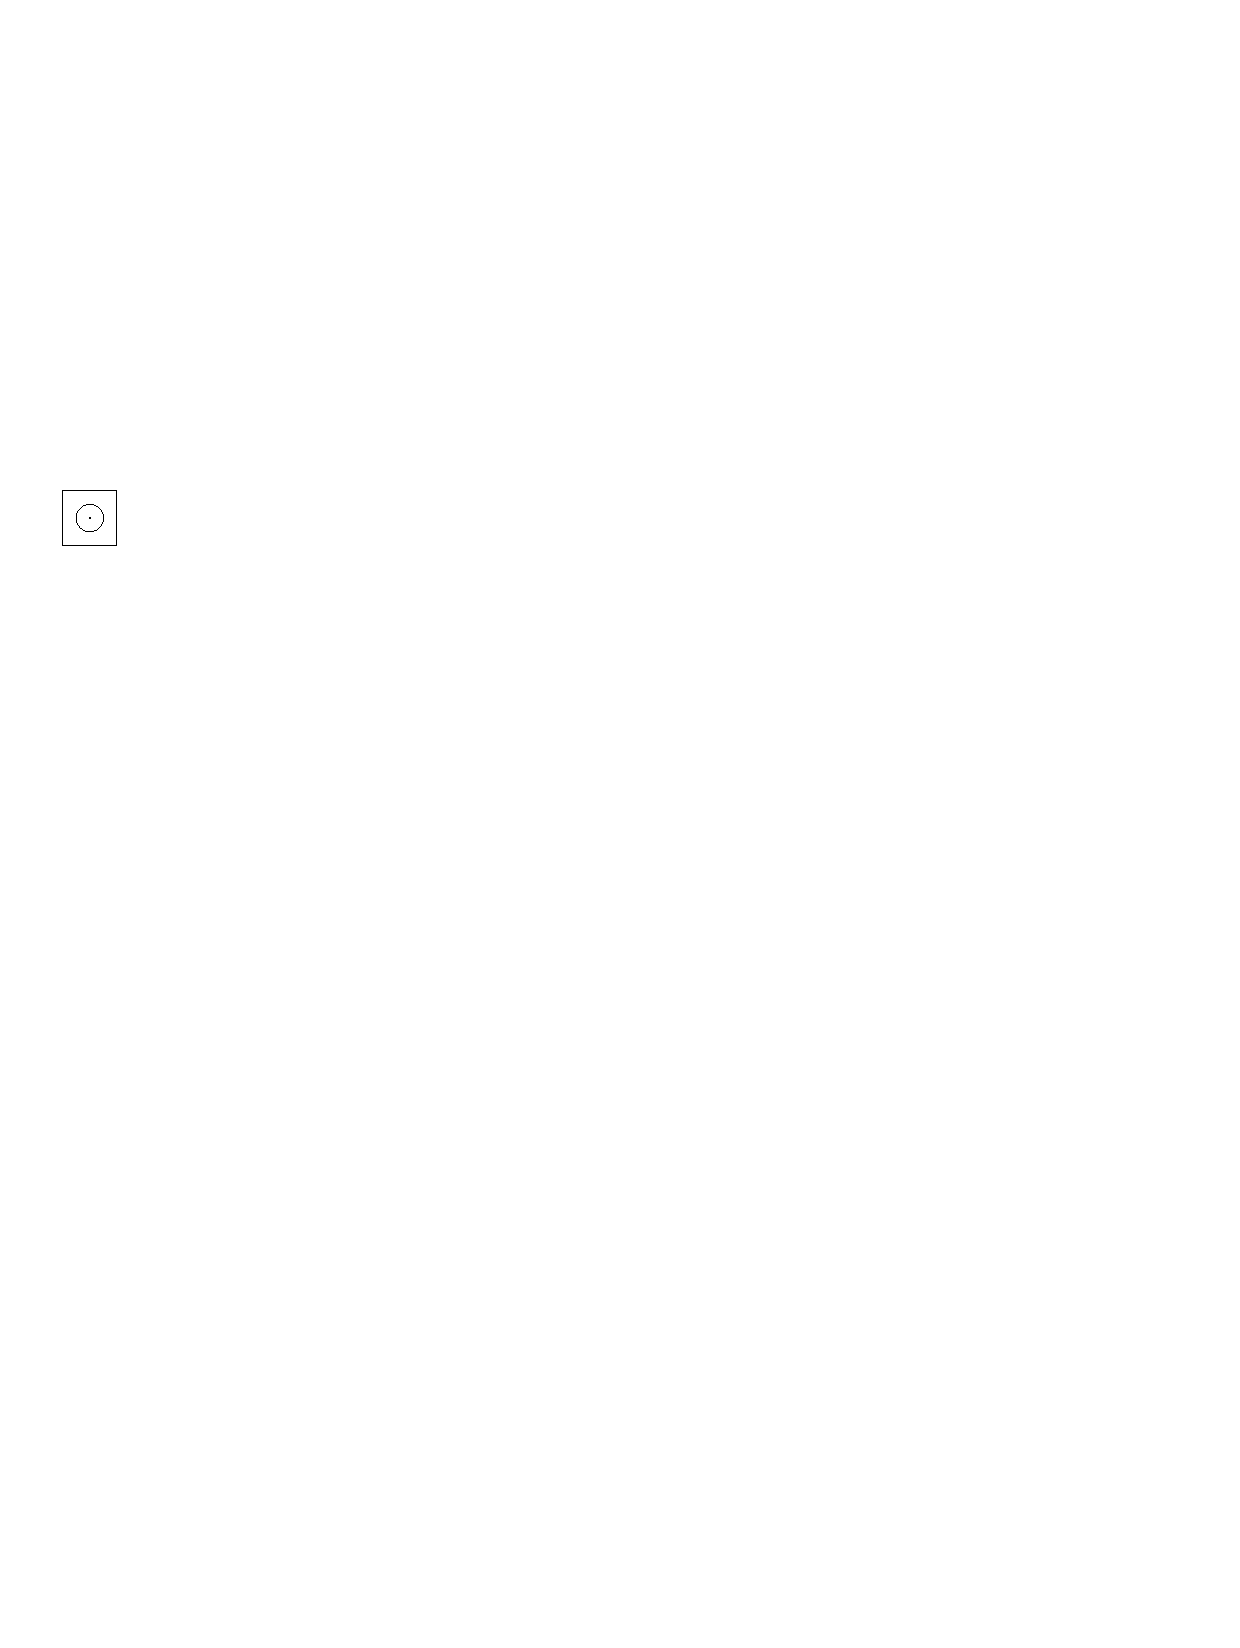
\includegraphics[scale=2]{img/sez_urto_p10}
\end{wrapfigure}
cada dentro il cerchietto è pari alla probabilità che questa particella venga diffusa. Quindi si può immaginare che una particella incidente subirà diffusione se cadrà dentro il cerchietto. La sezione d'urto viene anche detta \textit{sezione efficace di diffusione}. Nel caso limite di urto classico, $\sigma$ coincide con le dimensioni della particella bersaglio. Questo in realtà non si può mai verificare perché le particelle possono interagire senza venire a contatto.

Nella diffusione si possono avere sia diffusioni elastiche che anelastiche contemporaneamente (cioè alcune particelle subiscono diffusione elastica e altre anelastica). In questo caso si dice che la diffusione avviene secondo due canali. In questo caso $W$ è la somma sia di quella elastica che quella anelastica, cioè
\begin{equation}
 W = W_{\text{el}} + W_{\text{anel}}
\end{equation}
dove $W_{\text{el}}$ e $W_{\text{anel}}$ sono definite analogamente a $W$. Ovviamente si ha
\[
W_\text{el} = \sigma_\text{el}I n_b;\qquad W_\text{anel} = \sigma_\text{anel}I n_b
\]
\begin{align*}
 \sigma_\text{el} &= \text{sezione d'urto elastica}\\
 \sigma_\text{anel} &= \text{sezione d'urto anelastica}
\end{align*}
Essendo
\[
 W = \sigma I n_b \Rightarrow
\]
\begin{empheq}[box=\fbox]{equation}
 \sigma = \sigma_\text{el} + \sigma_\text{anel}
\end{empheq}

Un altro modo di definire la sezione d'urto è
\begin{align*}
N &= \text{numero di particelle diffuse nell'unità di tempo}\\
A_b &= \text{area della superficie bersaglio}\\
N &= W A_b
\end{align*}
Quindi si può scrivere
\[
N = \sigma I n_b A_b \Rightarrow N = \sigma I N_b
\]
dove $N_b$ è il numero totale di particelle bersaglio. Questo modo di definire $\sigma$ è comodo quando $N_b = 1$, infatti si avrà
\begin{empheq}[box=\fbox]{equation}
 \sigma = \frac{N}{I}
\end{empheq}
Questa è \textit{la probabilità che una singola particella incidente venga diffusa dal bersaglio}.

La frequenza di diffusione $W$ può anche interpretarsi come \textit{attenuazione d'intensità del fascio incidente}. Infatti $n = -\delta n_i$ che è il numero di particelle che il fascio incidente perde per unità di tempo per unità di superficie. Quindi
\[
n = -\delta n_i \Rightarrow \delta I = \delta n_i \Rightarrow
\]
\begin{empheq}[box=\fbox]{equation}
 W = -\delta I
\end{empheq}

\breaknote
Consideriamo\marginnote{17-11-1997} ora\footnote{Qui manca una frase che essenzialmente ripeteva quanto detto un rigo sopra, in quanto cambiando il giorno la lezione si riallaccia a quella precedente. \`E stata rimossa per migliorare la scorrevolezza. [NdT]} un fascio incidente che attraversa uno strato di materia. Sia $\Delta x= x- x_0$ lo spessore di questo strato e $\rho_b$ la densità di volume delle particelle bersaglio. Sia $I(x_0) = I(0)$ l'intensità iniziale del fascio incidente. Per calcolare $I(x)$ basta suddividere lo strato di spessore $\Delta x$ in strati infinitesimi di spessore $dx$. Il numero di particelle bersaglio per unità di area è $\rho_bdx$. La variazione di intensità dovuta al singolo strato è
\[
dI = -dW = -\sigma I \rho_bdx
\]
Si suppone che $\sigma$ non dipenda da $x$, cioè tutti gli strati hanno la stessa sezione d'urto. Integrando l'equazione si ha che
\[
\int\limits^{I(x)}_{I(0)} \frac{dI}{I} = -\int\limits^x_0 \sigma \rho_b dx \Rightarrow \ln[I(x)] - \lg[I(0)] = -\sigma\rho_b x \Rightarrow I(x) = I(0)e^{-\sigma\rho_bx}
\]
Si può anche scrivere nella forma
\begin{empheq}[box=\fbox]{equation}
 I(x) = I(0)e^{-\mu x}; \qquad \mu = \sigma\rho_b
\end{empheq}
$\mu$ si dice \textit{coefficiente di assorbimento} e ha le dimensioni di un inverso di una lunghezza. Da questa legge si determina che \textit{se $x\gg 1/\mu$, $I(x)$ diventa trascurabile}. Ad esempio i raggi cosmici non riescono a penetrare la crosta terrestre. Invece per i neutrini il coefficiente $\mu$ è molto piccolo e quindi un fascio di neutrini può attraversare tutta la terra senza subire grossa attenuazione. La sezione d'urto di solito si misura in \textit{barn} con la definizione
\begin{equation}
 1\text{ barn} = 10^{-24}\text{cm}^2
\end{equation}

Si è detto che la sezione d'urto totale si definisce come $\sigma = \sigma_\text{el} + \sigma_\text{anel}$. Analizziamo ora la probabilità che la diffusione avvenga in una particolare direzione. Consideriamo la direzione $(\theta,\phi)$ e l'angolo solido $d\Omega = \sin\theta d\theta d\phi$ e consideriamo il numero di particelle\footnote{Per coerenza con quanto detto prima, il numero di particelle si intende \textit{per unità di superficie e tempo}.} $dn$ che vengono diffuse\footnote{Sia elasticamente che anelasticamente. } nella direzione dell'angolo solido $d\Omega$. $dn$ sarà sempre proporzionale all'intensità del fascio incidente e alla densità di particelle bersaglio. Si può definire la frequenza
\[
dW = dn(\theta,\phi) = d\sigma(\theta,\phi)In_b = dW(\theta,\phi)
\]
moltiplicando e dividendo per $d\Omega$ si può scrivere\footnote{$d\sigma(\theta,\phi)$ è la sezione d'urto differenziale. }
\begin{equation}
dW = \frac{d\sigma}{d\Omega}In_bd\Omega
\end{equation}

Ovviamente deve esistere il legame con la sezione d'urto totale\footnote{Integrando sull'angolo solido. }
\begin{equation}
 \sigma = \int\limits^{4\pi}_0\frac{d\sigma}{d\Omega}d\Omega
\end{equation}
$\frac{d\sigma}{d\Omega}$ si può valutare\footnote{Come la $\sigma$ si distribuisca al variare dell'angolo solido. } sperimentalmente\footnote{Con contatori di particelle diffuse da spostare ai vari angoli. }. Si può sempre scrivere
\[
\frac{d\sigma}{d\Omega} = \frac{d\sigma_\text{el}}{d\Omega} + \frac{d\sigma_\text{anel}}{d\Omega}
\]

Consideriamo il caso in cui si abbia solo una particella bersaglio\footnote{In generale, se $N_b$ è il numero totale di particelle bersaglio $d\sigma = dN/(IN_b)$. }. Anche in questo caso si può definire la sezione d'urto differenziale
\[
d\sigma = \frac{dN}{I}, \qquad N_b = 1
\]
dove $dN$ è il numero di particelle incidenti che vengono diffuse nell'unità di tempo in un dato angolo solido $d\Omega$. Questa formula si può applicare al caso di una diffusione dovuta al potenziale elettrostatico\footnote{Modello di Rutherford. } generato da una carica fissa\footnote{$I$ è un flusso di particelle che si estende all'infinito. }.

L'importanza della diffusione è dovuta a due motivi: uno è che le interazioni della fisica nucleare e subnucleare  sono sempre a corto raggio e le sezioni d'urto possono fornire informazioni sulla struttura del bersaglio\footnote{Informazioni date dagli urti. }; il secondo motivo è che lo studio dettagliato di una interazione a corto raggio è molto più problematico rispetto a interazioni a raggio infinito. La trattazione è \textit{sempre quantistica e non esiste un corrispondente classico}, quindi l'analisi della sezione d'urto\footnote{Lo studio è abbastanza difficile. } è uno dei pochi strumenti che si hanno per studiare queste interazioni\footnote{Natura e meccanismo delle interazioni in gioco. }.

\section{Processi di decadimento}


Supponiamo che in un certo volume siano presenti delle particelle che hanno una certa probabilità di decadere. Supponiamo che queste particelle siano \textit{un insieme statistico}. Sia $N(t)$ il numero di particelle non ancora decadute al tempo $t$ e supponiamo che questo $N(t)$ sia sufficientemente grande in modo che si possa trattare come una grandezza continua (cioè $\lvert \delta N\rvert = 1 \ll N(t)$). All'istante $t + dt$ si avranno $N(t+dt)$ particelle non ancora decadute. Il numero di decadimenti nell'intervallo di tempo $dt$ è
\[
-dN(t) = N(t) - N(t+dt)
\]

La \textit{frequenza di decadimento} si definisce come
\begin{empheq}[box=\fbox]{equation}
 F(t) = -\frac{dN(t)}{dt}
\end{empheq}
questa rappresenta il numero di decadimenti nell'unità di tempo. Determiniamo ora la funzione $F(t)$ trattando i decadimenti come eventi casuali. Quindi il numero di decadimenti è proporzionale ad $N(t)$ con un coefficiente di proporzionalità che\footnote{Per l'omogeneità del tempo. } non può dipendere dal tempo. Quindi si può porre
\[
F(t) = -\frac{dN(t)}{dt} = \lambda N(t)
\]
$\lambda$ si dice \textit{costante di disintegrazione}\footnote{La probabilità di decadimento nell'unità di tempo. } (è l'analogo della sezione d'urto nei processi di diffusione). Ha le dimensioni di $t^{-1}$. Questa rappresenta la probabilità di decadimento nell'unità di tempo, cioè
\[
\lambda = -\frac{dN/dt}{N} = \textit{cost.}
\]
Tutto questo vale perché abbiamo fatto l'ipotesi di casualità dei decadimenti. Integrando l'equazione differenziale trovata per $N$ si ottiene che:
\begin{empheq}[box=\fbox]{equation}
 N(t) = N(0)e^{-\lambda t}
\end{empheq}
Da questa si ha
\begin{empheq}[box=\fbox]{equation}
 F(t) = \lambda N(0)e^{-\lambda t}
\end{empheq}
Questa legge esponenziale sembra essere valida per tutti i decadimenti\footnote{Quindi $F(t)$ non è una costante e ha un massimo per $t=0$. }

\section{Tempo di vita media}
Consideriamo\marginnote{19-11-1997}\footnote{Per la prima volta viene
  identificato il periodo storico del secondo Discente Ignoto, artefice degli
  Appunti negli Appunti. Infatti, accanto la data del '97 ne viene riportata una
  seconda: \textit{19/03/2007}.} sempre un volume in cui sono presenti delle
  particelle identiche che hanno una certa probabilità di decadere ($\lambda
$). Si definisce il \textit{tempo di vita media} di una particella
\begin{empheq}[box=\fbox]{equation}
 \tau = \frac{1}{\lambda}
\end{empheq}

Verifichiamo che effettivamente la vita media di una particella sia $1/\lambda$.
Consideriamo delle particelle che vivono da $0$ a $t$. Queste sono le particelle
che decadono nell'intervallo di tempo che va da $t$ a $t+dt$. Quindi si ha che
\[
dN'(t) = -dN(t) = \lambda N(t)dt = \lambda N(0)e^{-\lambda t}dt
\]
Questo è il numero di particelle che hanno vita pari a $t$. Per definizione la
vita media di una particella è
\begin{equation}
 \bar{t} = \frac{1}{N(0)}\int\limits^{+\infty}_0tdN'(t) = \frac{1}{N(0)}\int\limits^{+\infty}_0t\lambda N(t)dt = \int\limits^{+\infty}_0t\lambda e^{-\lambda t}dt = \frac{1}{\lambda} = \tau
\end{equation}

Si può verificare che se la frequenza di decadimento fosse costante ed uguale al
valore iniziale (cioè $F = \lambda N(0)=$ cost.) in questo caso $\tau$
rappresenterebbe il tempo in cui tutte le particelle sarebbero decadute. Infatti
\[
\int\limits^{N(t)}_{N(0)}dN = -\lambda N(0)t\Rightarrow N(t) = N(0)(1-\lambda t)
\]
Quindi si avrebbe $N(t) > 0$ per $t<\tau$ e $N(t) = 0$ per $t=\tau$.

Consideriamo il grafico della funzione $N(t)$ (\autoref{fig:decadimento_p15}):
\begin{enumerate}
 \item questa curva rappresenta $N(t) = N(0)e^{-\lambda t}$;
 \item questa curva rappresenta $N(t) = N(0)(1-\lambda t)$
\end{enumerate}
\begin{figure}[htbp]
\centering
\caption{Grafico delle due funzioni $N(t)$ considerate.}
\label{fig:decadimento_p15}
\begin{tikzpicture}[line cap=round,line join=round,>=stealth
  ,x=3.331070320176694cm,y=2.697038194702317cm]
  \draw[->,color=black] (-0.14,0) -- (2.56,0);
  \foreach \x in {,0.2,0.4,0.6,0.8,1,1.2,1.4,1.6,1.8,2,2.2,2.4}
  \draw[shift={(\x,0)},color=black] (0pt,2pt) -- (0pt,-2pt);
  \draw[->,color=black] (0,-0.17) -- (0,1.68);
  \foreach \y in {,0.2,0.4,0.6,0.8,1,1.2,1.4,1.6}
  \draw[shift={(0,\y)},color=black] (2pt,0pt) -- (-2pt,0pt);
  \clip(-0.14,-0.17) rectangle (2.56,1.68);
  \draw[smooth,samples=100,domain=0.0:2.5574449791162808]
  plot(\x,{2.718281828^(2*(\x)-4*(\x))});
  \draw[smooth,samples=100,domain=0.0:0.5] plot(\x,{1-2*(\x)});
  \draw (-0.09,1.68) node[anchor=north] {$N$};
  \draw (0.03,1.11) node[anchor=north west] {$N_0$};
  \draw (0.47,0.51) node[anchor=north west] {$1$};
  \draw (0.3,0.32) node[anchor=north] {$2$};
  \draw (0.48,0.03) node[anchor=north west] {$\tau$};
  \draw (2.03,-0.01) node[anchor=north west] {$t$};
  \begin{scriptsize}
	\fill [color=\MinorColor] (0,1) circle (1.5pt);
	\fill [color=\MinorColor] (0.5,0) circle (1.5pt);
  \end{scriptsize}
\end{tikzpicture}

\end{figure}
Quindi graficamente è possibile determinare $\tau$ considerando l'intersezione
con l'asse delle $x$ della retta tangente a $N(t) = N(0)e^{-\lambda t}$ nel
punto $t=0$. Definiamo\marginnote{Tempo di dimezzamento} ora il \textit{tempo di
dimezzamento}, cioè il tempo in cui il numero di particelle non decadute è
uguale alla metà del numero iniziale di particelle. Se indichiamo con $T$ il
tempo di dimezzamento si deve avere
\begin{equation}
 N(T) = \frac{1}{2}N(0) = N(0)e^{- T/\tau} \Rightarrow \frac{1}{2} = e^{-T/\tau} \Rightarrow T = \ln(2)\tau\approx 0.69\tau
\end{equation}

Tutte queste considerazioni teoriche sono una buona approssimazione della realtà
se la velocità delle particelle sono piccole rispetto a $c$, cioè se si è fuori
da ambiti relativistici\footnote{Oppure particelle ferme.}.

Vediamo ora come si definiscono questi parametri nel caso in cui le particelle
hanno una velocità $v$ non trascurabile rispetto a $c$. Quindi per $t$ e $T$ si
ha\footnote{Dipendono dal tipo di decadimento (interazione) e dalla velocità.}
\begin{align}
 \tau(v) &= \frac{\tau(0)}{\sqrt{1-v^2/c^2}}\\
 T(v) &= \frac{T(0)}{\sqrt{1-v^2/c^2}}
\end{align}
$\tau(v)$ è la vita media nel sistema in cui le particelle sono a velocità $v$,
$\tau(0)$ è la vita media nel sistema di riferimento in cui le particelle sono
ferme. Lo stesso vale per $T(v)$ e $T(0)$ e per $\lambda(v)$ e $\lambda(0)$. Per
$\lambda$ si ha
\begin{equation}
 \lambda(v) = \lambda(0)\sqrt{1-v^2/c^2}
\end{equation}
Quindi se una particella\footnote{Ad esempio i \textit{muoni}. } ha una vita
media piccola, se questa particella si trova a velocità $v\approx c$ la sua vita
media può aumentare notevolmente\footnote{$\tau$ è minimo nel \textsc{SR}
solidale alle particelle. }.

\chapter{Cenni di relatività}
\section{Energia cinetica relativistica}
I processi dinamici nucleari e subnucleari sono governati dalla legge $E_0 = mc^2$ dove $m$ è la massa a riposo. Se l'oggetto è in moto questa legge diventa
\[
E(v) = \frac{mc^2}{\sqrt{1-v^2/c^2}} = \gamma mc^2
\]
dove si è definito $\gamma = 1/\sqrt{1-v^2/c^2}$. Ovviamente $E(v=0) = E_0$. L'espressione $E(v)$ contiene l'energia totale dell'oggetto. Quindi $E(v)$ è la somma dell'energia cinetica e dell'energia a riposo, quindi si può scrivere
\begin{empheq}[box=\fbox]{equation}
T = E(v) - E_0 = mc^2(\gamma(v)-1)
\end{empheq}

Se $v\ll c$ si trova $T \approx \frac{1}{2}mv^2$. Questo risultato si ottiene sviluppando $\gamma (v)$ in serie di potenze di $v/c$, cioè arrestandosi al secondo ordine
\[
\gamma(v) \approx 1 + \frac{1}{2}\frac{v^2}{c^2}
\]
Quest'espressione di $T(v)$ si può trovare equivalentemente dal teorema dell'energia cinetica\footnote{$T$ = lavoro di una forza esterna per portare un corpo da $v =0$ a $v=v_0$. }. In fisica nucleare e subnucleare l'energia si esprime di solito in MeV\footnote{Un elettronvolt è l'energia cinetica di un elettrone accelerato da una differenza di potenziale pari a un volt. [NdT]} (1 eV = \SI{1.6e-19}{J} = \SI{1.6e-12}{erg}). Valutiamo ad esempio l'energia a riposo dell'elettrone, del protone e del neutrone in \autoref{tab:en_riposo}.
\begin{table}[htbp]
\centering
\caption{Energie a riposo di elettrone, protone e neutrone.}
\label{tab:en_riposo}
\begin{tabular}{cS[table-format=3.1]}
\toprule
Particella & {Energia (MeV)}\\
\midrule
$m_ec^2$ & 0.5\\
$m_pc^2$ & 938.2\\
$m_nc^2$ & 939.5\\
\bottomrule
\end{tabular}
\end{table}

La definizione relativistica di quantità di moto è
\begin{empheq}[box=\fbox]{equation}
 \vec{P} = \gamma(v) m\vec{v}
\end{empheq}
e di solito si indica $\gamma m$ \textit{massa effettiva} o massa relativistica. L'energia e la quantità di moto sono le componenti di un quadrivettore nello spazio di Minkowski\footnote{Lo spazio con la metrica descritta da $ds^2 = (cdt)^2 - dx^2 - dy^2 - dz^2$. }. Il modulo quadro di questo vettore è
\begin{empheq}[box=\fbox]{equation}
 P^2 = \frac{E^2}{c^2} - p^2;\qquad \vec{P} \equiv (\frac{E}{c}, \vec{p}) \tag{Quadrimpulso della particella}
\end{empheq}
dove si è adottata la metrica $ds^2 = (cdt)^2 - dx^2 - dy^2 - dz^2$. Sappiamo che i \textit{moduli di quadrivettori sono invarianti}\footnote{Restano invarianti per rotazioni, ovvero per cambiamento del SR. }, quindi $P^2 = \text{cost.}$ al variare del SR. Nel sistema in cui la particella è ferma si ha che $P^2 = E^2/c^2 = m^2c^2$. Quindi si ha \textit{sempre}
\begin{empheq}[box=\fbox]{equation}
 P^2 = \frac{E^2}{c^2} - p^2 = m^2c^2
\end{empheq}

Il fattore adimensionale $\gamma (v)$ rappresenta un utile parametro per valutare se è necessario o meno usare una trattazione relativistica. Il caso classico si ha per $\gamma = 1$, quindi se consideriamo il parametro $\gamma - 1$ questo ci da una stima dell'errore relativo che si ha usando una trattazione non relativistica. Infatti
\[
\gamma - 1 = \frac{\gamma m - m}{m}
\]
che è un errore relativo sulla massa.

\breaknote
Dalla\marginnote{21-11-1997} definizione relativistica dell'energia cinetica segue che il parametro $\gamma -1$ si può anche scrivere come
\begin{empheq}[box=\fbox]{equation}
 \gamma - 1 = \frac{T}{E_0} = \frac{\text{energia cinetica}}{\text{energia a riposo}}
\end{empheq}
Ad esempio in fisica nucleare per l'elettrone si ha
\[
T_e: [1\text{MeV}, 10\text{MeV}]
\]
quindi per l'elettrone si deve usare una trattazione relativistica. Infatti si ha
\[
0.2 \leq \gamma - 1 \leq 20
\]

Per il protone ed il neutrone energie cinetiche fino a 10MeV consentono una trattazione classica, infatti si ha 
\[
\gamma - 1  \lesssim 0.01 = 1\%
\]

\section{Energia di soglia}
Passiamo ora al concetto di \textit{energia di soglia}. Consideriamo un processo
dinamico in cui particelle più leggere si uniscono per dare origine a particelle
più pesanti. Vediamo in questo caso l'importanza del principio di equivalenza
fra massa ed energia. Consideriamo una particella $M$ bersaglio e una particella
$m$ che collide con $M$ ($m<M$ sono masse a riposo). Sia $M'$ la massa del
sistema che si genera dall'unione di $m$ e $M$. Questo sistema può essere
costituito da una sola particella o da $n$ particelle $M_1', M_2',...,M_n'$.
In questo caso la massa $M'$ si definisce come
\begin{equation}
 M' = \frac{E_\text{CM}}{c^2}; \qquad E_\text{CM} = \text{energia nel sistema del centro di massa}
\end{equation}

In generale, così definito $M'$, si ha che
\begin{equation}
 M' \geq M_1' + \cdots + M_n' > m+M
\end{equation}
L'eguaglianza si ha solo se le $M_i'$ sono tutte a riposo. Infatti in generale si ha
\begin{empheq}[box=\fbox]{equation}
 M' = E_\text{CM}/c^2 = \gamma(v_{1,\text{CM}}')M_1' + \cdots + \gamma(v_{n,\text{CM}}')M_n'; \qquad \gamma(v_{i,\text{CM}}) \geq 1
\end{empheq}
Dato quindi un processo di reazione di questo tipo si dice energia di soglia del processo l'energia minima $E_s$ che la particella incidente di massa $m$ deve avere affinché avvenga questo determinato processo. L'energia di soglia ovviamente deve essere tale che $M'$ assuma il suo valore minimo, cioè deve essere
\[
M' = M_1' + \cdots + M_n'
\]
Questa è la definizione di $E_s$. Vediamo adesso come si calcola.

Consideriamo il quadrimpulso delle particelle iniziali. Il suo modulo è
\begin{equation}
\label{eq:p_mod}
P^2_\text{tot} = \frac{(E + Mc^2)^2}{c^2} - p^2 = \frac{E^2}{c^2} + M^2c^2 + 2EM - p^2 = m^2c^2 + M^2c^2 + 2EM
\end{equation}
dove
\begin{itemize}
 \item[$p$] è il momento di $m$;
 \item[$E$] è l'energia di $m$;
 \item[$Mc^2$] è l'energia di $M$.
\end{itemize}
Da questo si vede che $P^2_\text{tot}$ è funzione solo di $E$. Consideriamo ora il modulo quadro del quadrimpulso finale
\[
P^{'2}_\text{tot} = M^{'2}c^2
\]
Per la conservazione del modulo quadro del quadrimpulso si deve avere che
\[
P^2_\text{tot}(E) = P^{'2}_\text{tot} = M^{'2}c^2
\]
Il valore di $E_s$ è quello tale che
\[
P^2_\text{tot}(E) = M^{'2}_\text{min}c^2 = (M_1' + \cdots + M_n')^2c^2
\]
e in forma esplicita, confrontata con \eqref{eq:p_mod}, questa equazione dà
\begin{empheq}[box=\fbox]{equation}
\label{eq:en_soglia}
 E_s = \frac{M^{'2}_\text{min} - M^2 - m^2}{2M}c^2
\end{empheq}
Nel caso particolare in cui il sistema finale sia costituito da una sola particella di massa $M'$ si ha
\[
E_s = \frac{M^{'2} - M^2 - m^2}{2M}c^2
\]

Applichiamo il concetto di energia di soglia al processo di formazione di una coppia elettrone-positrone. Ad esempio consideriamo la reazione
\begin{equation}
 \gamma + N \rightarrow e^+ + e^- + N
\end{equation}
dove $N$ è un nucleo. La presenza di $N$ \textit{è necessaria per garantire la conservazione della quantità di moto}. Infatti, se $N$ non fosse presente, si avrebbe
\[
\vec{P}_\text{in} = \vec{P}_\gamma \neq 0;\quad \vec{P}_\text{fin} = \vec{P}_{e^-} + \vec{P}_{e^+} = 0
\]
$\vec{P}_\text{fin}$ è nullo perché ci siamo posti nel sistema del centro di massa della coppia elettrone-positrone.

Calcoliamo ora l'energia di soglia relativa a questo processo. Sia $M_N$ la massa del nucleo, $m_e$ la massa del positrone e dell'elettrone. Nella \eqref{eq:en_soglia} si devono fare le seguenti sostituzioni
\[
M = M_N;\quad M'_\text{min} = M_N + 2m_e;\quad m = m_\gamma = 0
\]
Da queste si ottiene
\begin{equation}
 E_s = \frac{(M_n + 2m_e)^2 - M_N}{2M_N}c^2 = 2m_ec^2\left[1+\frac{m_e}{M_N}\right]
\end{equation}
Questa è l'energia minima che un fotone deve avere affinché da un urto con un nucleo si generi una coppia elettrone-positrone. Dall'espressione si deduce che $E_s > 2m_ec^2$ che è l'energia a riposo della coppia $e^+$-$e^-$. Questo è dovuto al fatto che dopo l'urto si avrà una energia cinetica sia del nucleo che di $e^+$ ed $e^-$. Però dal momento che $M_N\gg m_e$ si ha praticamente $E_s \approx 2m_ec^2$. Quindi le particelle $e^+$ ed $e^-$ sono strettamente a riposo rispetto al nucleo. Al limite si può assumere che la massa del nucleo sia infinita in modo che il nucleo non acquisti energia cinetica ed $E_s = 2m_ec^2$. In questa approssimazione la coppia $e^+$-$e^-$ è ferma. Se l'energia $E$ iniziale è maggiore di $E_s$ si ha un'energia cinetica della coppia $e^+$-$e^-$. Se $E$ continua ad aumentare si arriverà all'energia di soglia per il processo di creazione di due coppie elettrone-positrone.

\section{Energia di legame e difetto di massa}
Un'altra\marginnote{24-11-1997} conseguenza del principio di equivalenza fra
massa ed energia è il legame tra difetto di massa ed energia di legame. Sia $M$
la massa di una particella. Supponiamo che $M$ decada spontaneamente in due
particelle di massa $m_1$ e $m_2$. Per quanto detto prima si deve avere
\begin{align*}
M &> m_1 + m_2\\
Mc^2 &= \gamma(v_1) m_1c^2 + \gamma(v_2) m_2c^2
\end{align*}
Questo nel caso in cui $M$ decada spontaneamente. Supponiamo ora che $M$ sia
stabile e cioè non decada spontaneamente. Si definisce \textit{energia di
legame} l'energia minima che si deve fornire affinché $M$ si scinda in $m_1$ e
$m_2$. Definiamo le energie a riposo
\begin{equation}
 E_0 = Mc^2;\quad E_{01} = m_1c^2; \quad E_{02} = m_2c^2
\end{equation}
Se $\Delta E_0$ è l'energia di legame si deve avere per definizione
\begin{equation}
\Delta E_0 + E_0 = E_{01} + E_{02} \Rightarrow \Delta E_0 = (E_{01} + E_{02}) - E_0
\end{equation}
Per ipotesi deve essere $E_0 > 0$, quindi $E_0 < E_{01} + E_{02}$. A questo
punto applichiamo l'equivalenza fra massa ed energia e si può dedurre che $M <
m_1 + m_2$.

Quindi la \textit{particella $M$ stabile} ha massa inferiore alla somme delle
masse delle particelle che la compongono. Si definisce \textit{difetto di massa}
\begin{equation}
 \Delta M = (m_1 + m_2) - M = \text{Difetto di massa}
\end{equation}
e ovviamente
\begin{equation}
\Delta M = \frac{\Delta E_0}{c^2}
\end{equation}
Questo risultato trova applicazione nei nuclei stabili. \textit{La massa di un
nucleo stabile è minore delle masse di protoni e neutroni che lo compongono}.
Consideriamo ad esempio il nucleo d'elio
\[
  2m_p + 2m_n \approx 3755 \ \dfrac{\text{MeV}}{c^2}
\]
mentre il valore sperimentale della massa del nucleo d'elio è
\begin{align*}
M_\text{He} &\approx 3727\text{MeV/c}^2\\
\Delta M &\approx 28\text{MeV/c}^2 \Rightarrow \Delta E_0 \approx 28\text{MeV}
\end{align*}
Quindi misurando la massa di un nucleo si può dedurre $\Delta E_0$ e quindi le forze che tengono uniti i nucleoni.

\chapter{Cenni di meccanica quantistica}

\section{Statistiche di Fermi-Dirac e Bose-Einstein}

Se $\psi(\vec{r},t)$ è la funzione d'onda di una particella, allora
$\abs{\psi(\vec{r},t)}^2d^3r$ è la probabilità che all'istante $t$ la particella
si trovi nel volumetto $d^3r$ centrato nel punto $\vec{r}$. Questa funzione
$\psi(\vec{r},t)$ è soluzione dell'equazione di Schr\"odinger
\begin{equation}
 i\hslash \frac{\partial}{\partial t}\psi(\vec{r},t) = H \psi(\vec{r},t)
\end{equation}

Consideriamo due particelle, 1 e 2, e sia $\psi(1,2,t)$ la funzione d'onda. Se
non consideriamo lo spin questa si può scrivere come $\psi(\vec{r}_1, \vec{r}_2,
t)$. Se le due particelle non sono interagenti si ha
\[
H(1,2) = H(1) + H(2)
\]
ovvero l'hamiltoniana del sistema è uguale alla somma delle hamiltoniane delle
due particelle. Per quanto detto si avrà che
\[
\psi(1,2,t) = \psi_a(1,t)\cdot \psi_b(2,t)
\]
dove $\psi_a$ e $\psi_b$ sono soluzioni dell'equazione di Schr\"odinger con
$H(1)$ e $H(2)$. La funzione $\psi_a$ rappresenta lo stato quantistico della
particella 1 e $\psi_b$ lo stato della particella 2. In \textit{generale}
$\psi_a \neq \psi_b$. Per quanto definito si avrà per la probabilità
\[
\abs{\psi(1,2,t)}^2\cdot d^3r_1\cdot d^3r_2 = \abs{\psi(1,t)}^2d^3r_1\cdot
\abs{\psi(2,t)}^2d^3r_2
\]
Questa è la probabilità di trovare simultaneamente la particella 1 in
$\vec{r}_1$ e la particella 2 in $\vec{r}_2$. Quanto fatto ha senso se le due
particelle sono distinguibili l'una dall'altra. Solo in questo caso infatti si
può porre una corrispondenza biunivoca $1\leftrightarrow\psi_a$ e
$2\leftrightarrow\psi_b$. Questa corrispondenza perde di significato quando le
particelle sono identiche in quanto \textit{dal punto di vista quantistico sono
indistinguibili, a meno che le loro funzioni d'onda non siano definite in domini
spaziotemporali con intersezione nulla}. Quando questo non avviene le particelle
sono indistinguibili.

Analizziamo le conseguenze di questa indistinguibilità mantenendo però valida
l'ipotesi di due particelle non interagenti. Sia $\psi(1,2,t)$ la loro funzione
d'onda. Deve essere che
\[
\psi(1,2,t) \neq \psi_a(1,t)\psi_b(2,t)
\]
perché non si può stabilire quale particella si trovi nello stato $\psi_a$ e
quale nello stato $\psi_b$. Cioè la funzione d'onda deve contenere
contemporaneamente i termini $\psi_a(1,t)\psi_b(2,t)$ e
$\psi_a(2,t)\psi_b(1,t)$. Introduciamo \textit{l'operatore di scambio} $P_{1,2}$
il cui unico effetto è quello di scambiare le due particelle (cioè le loro
coordinate), cioè si definisce
\begin{equation}
\begin{rcases}
P_{1,2}\psi(1,2,t) &= \psi(2,1,t)\\
P_{1,2} \psi_i(1,t) &= \psi_i(2,t)\\
P_{1,2} \psi_i(2,t) &= \psi_i(1,t)
\end{rcases}\text{con }i=a,b
\end{equation}
Se applichiamo questo operatore, questo \textit{non potrà provocare alcun
cambiamento osservabile}. Quindi deve essere
\[
\abs{\psi(1,2,t)}^2 = \abs{\psi(2,1,t)}^2
\]
Questa uguglianza implica che
\[
P_{1,2}\psi(1,2,t) \equiv \psi(2,1,t) = \eta\psi(1,2,t)\qquad\text{con }\abs{\eta}^2 = 1
\]
Poiché l'assegnazione dei numeri 1 e 2 è puramente convenzionale deve essere
verificata la relazione
\[
P_{1,2}\psi(2,1,t) \equiv \psi(1,2,t) = \eta\psi(2,1,t)
\]
Da queste due si deduce che $\eta^2=1\Rightarrow\eta=\pm 1$. Per la funzione
d'onda $\psi$ si può porre in definitiva che
\begin{equation}
\psi(1,2,t)\propto[\psi_a(1,t)\psi_b(2,t) + \eta\psi_a(2,t)\psi_b(1,t)]
\end{equation}

\breaknote
Nel\marginnote{26-11-1997} caso in cui le particelle identiche siano interagenti
non sarà più possibile scrivere le loro funzioni d'onda in forma fattorizzata,
questo perché l'Hamiltoniana in questo caso è del tipo
\[
H(1,2) = H(1) + H(2) + V(1,2)
\]
Continua però a sussistere l'indistinguibilità, quindi deve essere sempre
verificato che
\[
P_{1,2}\psi(1,2,t) \equiv \psi(2,1,t) = \eta\psi(1,2,t)\qquad\text{con }\eta =\pm 1
\]
Si può concludere in modo generale che \textit{la funzione d'onda di due
particelle identiche è simmetrica o antisimmetrica rispetto allo scambio delle
coordinate}. Questa è infatti una proprietà intrinseca, rimane cioè invariata
nel tempo. Infatti si ha
\begin{align*}
 \psi(1,2,t+dt) &= \psi(1,2,t) + \frac{\partial}{\partial t}\psi(1,2,t)dt\\
 i\hslash \frac{\partial}{\partial t}\psi(1,2,t) &= H \psi(1,2,t)
\end{align*}
e $H$ è ovviamente invariante \textit{per lo scambio delle due particelle}, cioè
$H(1,2) = H(2,1)$. Tenuto conto di questa proprietà segue dall'equazione di
Schr\"odinger
\begin{equation}
 i\hslash \frac{\partial}{\partial t}\psi(2,1,t) = H \psi(2,1,t) = \eta H \psi(1,2,t) = \eta i\hslash \frac{\partial}{\partial t}\psi(1,2,t)
\end{equation}
Quindi $\frac{\partial}{\partial t}\psi(2,1,t) = \eta \frac{\partial}{\partial
t}\psi(1,2,t)$. Da queste considerazioni si deriva che $\eta$ \textit{non può
essere funzione del tempo}. Quando $\eta = 1$ si dice che le due particelle
identiche obbediscono alla \textit{statistica di Bose-Einstein}; quando $\eta =
-1$ le due particele identiche obbediscono alla \textit{statistica di
Fermi-Dirac}.
\begin{empheq}[box=\fbox]{align}
 \psi(1,2,t) &= \psi(2,1,t)\qquad\text{statistica di \textit{Bose-Einstein}}\\
 \psi(1,2,t) &=-\psi(2,1,t)\qquad\text{statistica di \textit{Fermi-Dirac}}
\end{empheq}

Le particelle del primo tipo si chiamano
\textit{bosoni}. Le particelle del secondo si chiamano \textit{fermioni}. Le
particelle del secondo tipo sono soggette al principio di esclusione di Pauli.
Infatti se due fermioni identici non interagenti\footnote{Se due particelle
  fossero invece interagenti, non avrebbe senso parlare di principio di Pauli in
  quanto non si potrebbe parlare di stato di \textit{una} singola particella.}
  avessero lo stesso stato quantico allora la loro funzione d'onda complessiva
  sarebbe
\[
\psi(1,2)\propto[\psi_a(1)\psi_b(2) - \psi_a(2)\psi_b(1)] \equiv 0
\]
Empiricamente sappiamo che si comportano come bosoni tutte le particelle che
hanno spin pari a un multiplo intero di $\hslash$. Quando lo spin è un multiplo
semi-intero di $\hslash$ le particelle si comportano come fermioni.

Consideriamo adesso un insieme di $N$ particelle identiche non interagenti. Il
generico stato in cui una particella può trovarsi sia
$\psi_{k_i}\;(i=1,\dots,N)$. Se le particelle fossero distinguibili si potrebbe
assegnare a ciascuna di esse un ben determinato stato e la funzione complessiva
sarebbe
\[
\psi(1,\dots,N) = \psi_{k_1}(1)\psi_{k_2}(2)\cdots\psi_{k_N}(N)
\]
Se invece le particelle sono indistinguibili, uno o più scambi di particelle non
possono portare a cambiamenti del sistema. In questo caso deve essere verificato
che
\begin{equation}
 P_{ij}\psi_{k_i}(i)\psi_{k_j}(j) = \psi_{k_i}(j)\psi_{k_j}(i)
\end{equation}
Se si tratta di fermioni, la funzione complessiva sarà antisimmetrica per un
numero dispari di scambi e simmetrica per un numero pari di scambi. Se si tratta
invece di bosoni, la funzione d'onda complessiva sarà sempre simmetrica per un
numero qualsiasi di scambi effettuati.

Consideriamo l'insieme di indici $(1,2,\dots,N)$ e una generica permutazione
$P\equiv (P_1,P_2,\dots,P_N)$. Il numero delle possibili permutazioni è $N!$.
Ciascuna permutazione $P$ si ottiene dalla successione iniziale per mezzo di un
numero di scambi $n_P$. Quindi un sistema di $N$ particelle identiche non
interagenti, che siano dei fermioni, si può descrivere con una funzione d'onda
complessiva del tipo\footnote{I pedici $FD$ e $BE$ stanno per Fermi-Dirac e
Bose-Einstein rispettivamente. [NdT]}
\begin{equation}
 \psi_{FD} \propto \sum\limits_P(-1)^{n_P}\psi_{k_1}(P_1)\psi_{k_2}(P_2)\cdots\psi_{k_N}(P_N)
\end{equation}
Nel caso di bosoni invece si ha
\begin{equation}
 \psi_{BE} \propto \sum\limits_P\psi_{k_1}(P_1)\psi_{k_2}(P_2)\cdots\psi_{k_N}(P_N)
\end{equation}

Queste funzioni sono definite a meno di un fattore moltiplicativo. Per trovare
tale fattore basta considerare l'interpretazione probabilistica della funzione
d'onda. Assumiamo che le singole funzioni d'onda siano già normalizzate, cioè
\[
\int_V \abs{\psi_{k_i}(P_i)}^2d^3r_{P_i} = \int_V \abs{\psi_{k_i}(i)}^2d^3r_{i}
= 1
\]
Un'analoga condizione di normalizzazione deve valere per la funzione d'onda
complessiva, cioè deve essere verificato che
\[
\int_V \abs{\psi_{FD}}^2d^3r_1\, d^3r_2\,\cdots\, d^3r_N = \int_V
\abs{\psi_{BE}}^2d^3r_1\, d^3r_2\,\cdots\, d^3r_N = 1
\]
Facciamo l'ipotesi che sia $\psi_{k_i} \neq \psi_{k_j}$ per $i\neq j$, cioè che
gli stati siano tutti diversi. Questa ipotesi è obbligatoria se si considerano
fermioni identici. Comunque assumiamo questo vero anche se le particelle sono
bosoni. Sotto queste ipotesi vale anche una condizione di ortonormalità fra gli
stati, cioè
\[
 \int_V \psi^*_{k_i}(P_i)\psi_{k_j}(P_i)\, d^3r_{P_i} = \int_V
 \psi^*_{k_i}(i)\psi_{k_j}(i)\, d^3r_{i} = \delta_{ij}
\]
Tenuto conto di queste considerazioni, la condizione di normalizzazione della
funzione d'onda complessiva risulta verificata se si pone
\begin{empheq}[box=\fbox]{align}
 \psi_{FD} &=
 \frac{1}{\sqrt{N!}}\sum\limits_P(-1)^{n_P}\psi_{k_1}(P_1)\psi_{k_2}(P_2)\cdots\psi_{k_N}(P_N)\\
 \psi_{BE} &= \frac{1}{\sqrt{N!}}\sum\limits_P\psi_{k_1}(P_1)\psi_{k_2}(P_2)\cdots\psi_{k_N}(P_N)
\end{empheq}
Nel caso in cui $N=2$, cioè se si hanno solo due particelle identiche, si ha che
\begin{align}
 \psi_{FD} &= \frac{1}{\sqrt{2}}[\psi_{k_1}(1)\psi_{k_2}(2) - \psi_{k_1}(2)\psi_{k_2}(1)]\\
 \psi_{BE} &= \frac{1}{\sqrt{2}}[\psi_{k_1}(1)\psi_{k_2}(2) + \psi_{k_1}(2)\psi_{k_2}(1)]
\end{align}
ricordando che questi fattori di noralizzazione ($1/\sqrt{N!}$) valgono sotto
l'ipotesi di stati tutti differenti.

\section{Funzione d'onda di una particella che decade}

In\marginnote{28-11-1997} meccanica quantistica lo stato di una particella
libera con quantità di moto ed energia ben definite si dice \textit{stato
stazionario} e la funzione d'onda che lo descrive è
\begin{equation}
 \phi(\vec{r},t) = \phi(\vec{r})\psi(t)\qquad\text{dove }\phi(\vec{r})\propto e^{\frac{i}{\hslash}\vec{p}\cdot\vec{r}}\quad\text{e}\quad\psi(t) = \psi(0)e^{-\frac{i}{\hslash}Et}
\end{equation}
Se la particella è a riposo $E=E_0=mc^2$, con $m$ massa della particella.
Ovviamente si ha che
\[
\abs{\psi(t)}^2 = \abs{\psi(0)}^2 = \text{costante}
\]
Supponiamo di normalizzare la funzione d'onda $\phi(\vec{r},t)$ in modo tale che
\[
\int_V\abs{\phi(\vec{r},t)}^2\, d^3r = \int_V\abs{\phi(\vec{r})}^2\, d^3r =
1\quad\text{dove si è posto }\abs{\psi(0)}^{2}=1
\]
$\abs{\psi(t)}^2 = \abs{\psi(0)}^2 = 1$ si interpreta come la probabilità che la
particell esista nel volume $V$ all'instante $t$. Essendo questa uguale a 1, la
particella risulta stabile.

\textit{Se invece la particella non fosse stabile non potrebbe essere}
$\abs{\psi(t)}=1$ verificata ad ogni $t$, quindi lo stato della particella non
potrà essere uno stato stazionario. Per il principio di indeterminazione tra
tempo ed energia deve essere
\[
\Delta E = \hslash/\tau
\]
dove $\tau$ è la vita media della particella. Questo è in accordo col fatto che
la particella non è in uno stato stazionario.

Si ha però che lo stato di una particella che decade si può in genere
approssimare ad uno \textit{stato quasi stazionario}. Cioè si può assumere che
l'andamento temporale della funzione d'onda sia
\begin{equation}
 \psi(t) = \psi(0)e^{-\frac{i}{\hslash}Et}
\end{equation}
dove però $E$ è una quantità complessa. In particolare si ha
\begin{empheq}[box=\fbox]{equation}
 E = \bar{E} - i\frac{\Gamma}{2}
\end{empheq}
dove $\bar{E}$ e $\Gamma$ sono numeri positivi. Con queste considerazioni la
funzione d'onda si può scrivere
\begin{equation}
 \psi(t) = \psi(0)\exp\left[-\frac{i}{\hslash}\bar{E}t - \frac{1}{2\hslash}\Gamma t\right]
\end{equation}
In questo caso si vede che la $\psi(t)$ è sostanzialmente diversa da quella
dello stato stazionario. Si vede che quanto più $\Gamma$ è piccolo, tanto più lo
stato si avvicina ad uno stato stazionario. Dal momento che
\[
E\longrightarrow\bar{E}\qquad\text{per }\Gamma\longrightarrow 0
\]
si può interpretare $\bar{E}$ \textit{come il valore medio dell'energia}, cioè l'energia può assumere valori nell'intervallo
\begin{equation}
 \left[\bar{E} - \frac{\Delta E}{2};\;\bar{E} + \frac{\Delta E}{2}\right]
\end{equation}
dove $\Delta E$ è l'incertezza data dal principio d'indeterminazione. In particolare \textit{se la particella è a riposo $\bar{E}$ ci da il valore medio della massa della particella}. Quindi \textit{una particella instabile non ha una massa ben definita}.

Consideriamo adesso la quantità $\Gamma$. Il modulo quadro di $\psi(t)$ è 
\begin{equation}
 \abs{\psi(t)}^2=\abs{\psi(0)}^2e^{-\frac{\Gamma}{\hslash}t} = e^{-\frac{\Gamma}{\hslash}t}
\end{equation}
dove si è posto $\abs{\psi(0)}^2 = 1$. $\abs{\psi(t)}^2$ ci deve sempre dare la probabilità che la particella esista al tempo $t$ nel volume $V$.

Per un insieme statistico di particelle identiche instabili sappiamo che il numero di particelle non ancora decadute all'istante $t$ è
\begin{equation}
 N(t) = N(0)e^{-\lambda t}
\end{equation}
quindi si può porre, per il significato probabilistico di $\abs{\psi(t)}^2$
\begin{equation}
 \abs{\psi(t)}^2 = N(t)/N(0)
\end{equation}
Da questa segue che
\[
e^{-\Gamma t/\hslash} = e^{-\lambda t}
\]
ovvero
\begin{empheq}[box=\fbox]{equation}
 \label{eq:largh_lvl_en}
 \Gamma = \hslash\lambda = \hslash/\tau = \Delta E
\end{empheq}
Tenendo conto del principio di indeterminazione si interpreta $\Gamma$ come l'indeterminazione minima dell'energia di una particella che decade. $\Gamma$ viene detta \textit{larghezza del livello energetico di una particella}. \`E logico aspettarsi che l'approssimazione di stato quasi stazionrio sia buona quando $\Gamma\ll\bar{E}$, cioè quando è possibile assegnare un valore di energia abbastanza preciso.

Questa condizione può essere vista anche sotto un altro aspetto, infatti possiamo scrivere
\begin{equation}
 \tau = \hslash/\Gamma \gg \hslash/\bar{E} = \bar{T}
\end{equation}
dove $\bar{T}2\pi$ è il periodo medio caratteristico di oscillazione della funzione d'onda della particella. Di conseguenza \textit{si può parlare di stato quasi stazionario quando la vita media della particella è molto più grande del periodo di oscillazione della funzione d'onda}.

Il decadimento di una particella può avvenire teoricamente o in un unico modo oppure in modi diversi. Ad esempio un atomo che si trova ad un livello energetico eccitato può avere un unico modo di decadere se esiste un solo livello più basso, mentre se esistono più livelli inferiori il decadimento può avvenire in modi diversi, con diversi stati finali.

Consideriamo il caso generale in cui siano $n$ il numero di possibili modi di decadere, ciascuno di questi caratterizzati dalla costante $\lambda_i(i=1,\dots,n)$. Si dice che in questo caso la particella ha $n$ canali di decadimento e $\lambda_i$ la probabilità di decadere nell'unità di tempo per il canale i-esimo. In questo caso si ha
\begin{equation}
 \lambda = \sum_i\lambda_i
\end{equation}
Per ciascun canale si può definire una larghezza parziale
\begin{equation}
 \Gamma = \hslash \lambda = \sum_i\Gamma_i
\end{equation}

Consideriamo un insieme statistico di particelle identiche con $n$ canali di decadimento. Si ha che
\begin{equation}
\frac{\Gamma_i}{\Gamma} = \frac{\lambda_i}{\lambda}
\end{equation}
è la percentuale di decadimenti nell'i-esimo canale. Questo si dice \textit{rapporto di diramazione} (= ``branching ratio''). Si definiscono pure i tempi parziali di vita media
\begin{equation}
 \tau_i = 1/\lambda_i
\end{equation}
Questi però possono contribuire all'effettivo tempo di vita media secondo la relazione
\begin{equation}
 \tau = 1/\lambda\Rightarrow \frac{1}{\tau} = \sum_i\frac{1}{\tau_i}\Rightarrow\tau<\tau_i\quad\forall i = 1,\dots,n
\end{equation}
